%%% Figure from: Schär, Fabian. "Blockchain Forks: A Formal Classification Framework and Persistency Analysis." (2020).

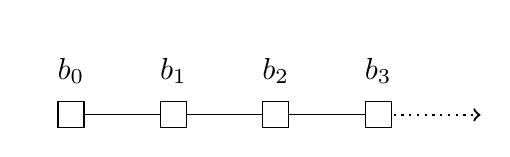
\begin{tikzpicture}[domain=1:10,scale=1.3, every node/.style={scale=1.1}]
\coordinate (o1) at (1,1);
\coordinate (o2) at (2,1);
\coordinate (o3) at (3,1);
\coordinate (o4) at (4,1);
\coordinate (o5) at (5,1);
\coordinate (o6) at (6,1);
\coordinate (o7) at (7,1);
\coordinate (o8) at (8,1);
\coordinate (o9) at (9,1);
\coordinate (o10) at (10,1);
\coordinate (n1) at (1,0.25);
\coordinate (n2) at (2,0.25);
\coordinate (n3) at (3,0.25);
\coordinate (n4) at (4,0.25);
\coordinate (n5) at (5,0.25);
\coordinate (n6) at (6,0.25);
\coordinate (n7) at (7,0.25);
\coordinate (n8) at (8,0.25);
\coordinate (n9) at (9,0.25);
\coordinate (n10) at (10,0.25);

  \draw[color=black] (o1) to[] (o2) to[] (o3) to[] (o4);
  \draw[color=black,thick, dotted, ->] (o4) to[] (o5);
  \node (rect) at (o1) [fill=white,draw,minimum width=0.3cm,minimum height=0.3cm] {};
  \node at (o1) [minimum width=1cm,minimum height=1cm,above] {${b}_0$};
  \node (rect) at (o2) [fill=white,draw,minimum width=0.3cm,minimum height=0.3cm] {};
  \node at (o2) [minimum width=1cm,minimum height=1cm,above] {${b}_1$};
  \node (rect) at (o3) [fill=white,draw,minimum width=0.3cm,minimum height=0.3cm] {};
  \node at (o3) [minimum width=1cm,minimum height=1cm,above] {${b}_2$};
  \node (rect) at (o4) [fill=white,draw,minimum width=0.3cm,minimum height=0.3cm] {};
  \node at (o4) [minimum width=1cm,minimum height=1cm,above] {${b}_3$};
\end{tikzpicture}
